\section{Lecture 7: The Discrete-Time Fourier Transform}

We begin by defining the \textbf{discrete-time Fourier transform} (DTFT)
%
\begin{equation}\label{eq::lecture_7_dtft}
  X(\omega) = \sum_{n=-\infty}^\infty x[n]\ex{-\im\omega n} \,.
\end{equation}
%
Note that while this expression is discrete in time, it is continuous
in frequency. However, while the continuous-time Fourier transform
has the frequency range $[-\infty,\infty]$, the DTFT is $2\pi$-periodic
as we've previously pointed out,
%
\begin{displaymath}
  X(\omega + 2\pi) = \sum_{n=-\infty}^\infty x[n]\ex{-\im(\omega+2\pi)n}
  = \sum_{n=-\infty}^\infty x[n]\ex{-\im\omega n}\ex{-\im 2\pi n}
  = \sum_{n=-\infty}^\infty x[n]\ex{-\im\omega n} = X(\omega) \,.
\end{displaymath}
%
So while the DTFT can be evaluated at any frequency, we must exercise
caution in only concerning ourselves with the range $[-\pi,\pi]$.
We'll also introduce the \textbf{discrete-time inverse Fourier transform}
(IDTFT) as
%
\begin{equation}
  x[n] = \frac{1}{2\pi}\int_{-\pi}^\pi\dx{\omega} X(\omega)\ex{\im\omega n} \,.
\end{equation}
%
We can prove that this is the inverse of \eqref{eq::lecture_7_dtft} by
%
\begin{align*}
  x[n] &= \frac{1}{2\pi}\int_{-\pi}^\pi\dx{\omega} X(\omega)\ex{\im\omega n}
  = \frac{1}{2\pi}\int_{-\pi}^\pi\dx{\omega} \sum_{m=-\infty}^\infty x[m]\ex{-\im\omega m}\ex{\im\omega n} \\
  &= \sum_{m=-\infty}^\infty \frac{x[m]}{2\pi}\int_{-\pi}^\pi\dx{\omega}\ex{\im\omega(n-m)}
  = \sum_{m=-\infty}^\infty \frac{x[m]}{2\pi}\delta_{mn}2\pi \\
  &= x[n] \,,
\end{align*}
%
as required. However, note that a sufficient condition for the interchange of
summation and integration on the second line is that $\sum_n|x[n]| < \infty$,
as per the Fubini-Tonelli theorem.
%
\begin{exmp}
  Consider the frequency response given by the top hate which is high over the
  interval $[-\omega_c,\omega_c]$, where $\omega_c < \pi$. Then
  %
  \begin{align*}
    x[n] &= \frac{1}{2\pi}\int_{-\pi}^\pi \dx{\omega}X(\omega)\ex{-\im\omega n}
    = \frac{1}{2\pi}\int_{-\omega_c}^{\omega_c} \dx{\omega}\ex{-\im\omega n}
    = \left. \frac{1}{2\pi\im n}\ex{-\im\omega n}\right|_{-\omega_c}^{\omega_c} \\
    &= \frac{1}{2\pi\im n} \left(\ex{\im\omega_c n} - \ex{-\im\omega_c n}\right)
    = \frac{1}{\pi n}\sin(\omega_c n) = \frac{\omega_c}{\pi}\sinc(\omega_c n) \,.
  \end{align*}
  %
  This function satisfies $\sum_n|x[n]|^2 < \infty$, but not $\sum_n|x[n]| < \infty$,
  which manifests itself as the Gibbs phenomenon since the interchange of summation
  and integration that was invoked in the proof of the IDTFT is no longer valid.
\end{exmp}
%
\begin{exmp}
  Let
  %
  \begin{displaymath}
    x[n] = \delta[n] \Longleftrightarrow X(\omega)
    = \sum_{n=-\infty}^\infty\delta[n]\ex{-\im\omega n} = 1 \,.
  \end{displaymath}
  %
  Now consider $X(\omega) = \delta(\omega)$. Recall that the DTFT is
  $2\pi$-periodic. What we mean by $X(\omega) = \delta(\omega)$ is that
  there is a delta function at every interval of $2\pi$:
  %
  \begin{displaymath}
    X(\omega) = \delta(\omega) \Longleftrightarrow x[n]
    = \frac{1}{2\pi}\int_{-\pi}^\pi\dx{\omega}X(\omega)\ex{\im\omega n} = \frac{1}{2\pi} \,.
  \end{displaymath}
  %
  So a delta function in the frequency domain is a constant in the time
  domain, and \textit{vice versa}, as before.
\end{exmp}
%
\begin{exmp}
  Consider a pulse in the time domain,
  %
  \begin{displaymath}
    x[n] = \left\{\begin{array}{ccl}
    1 & & -m \leq n \leq m \\
    0 & & \mathrm{otherwise}
    \end{array}\right. \,.
  \end{displaymath}
  %
  From the continuous Fourier transform of the top hat function, we expect
  something like a $\sinc$ for the DTFT. But $\sinc$ is not periodic, let alone
  $2\pi$-periodic. Consequently, we expect something like $\sinc$, but $2\pi$-periodic.
  The DTFT is
  %
  \begin{displaymath}
    \infsum{n}x[n]\ex{-\im\omega n} = \sum_{n=-m}^m \ex{-\im\omega n}
    = \ex{\im\omega m}\sum_{n=0}^{2m}\ex{-\im\omega n} \,.
  \end{displaymath}
  %
  With a little foresight, we'll find it prudent to evaluate
  $X(0) = 2m + 1$ before simplifying further. Next, from a table of finite sum
  expressions, we have
  %
  \begin{displaymath}
    \ex{\im\omega m}\sum_{n=0}^{2m}\ex{-\im\omega n}
    = \ex{\im\omega m}\left(
    \frac{1 - \ex{-\im\omega(2m+1)}}{1 - \ex{-\im\omega}}
    \right) \,.
  \end{displaymath}
  %
  Note that this expression is undefined at $\omega = 0$. We can force some
  sinusoids to appear in this expression by factoring out $\ex{-\im\omega\frac{2m+1}{2}}$
  in the numerator and $\ex{-\frac{\im\omega}{2}}$,
  %
  \begin{align*}
    X(\omega) &= \ex{\im\omega m}\left(
    \frac{1 - \ex{-\im\omega(2m+1)}}{1 - \ex{-\im\omega}}
    \right)
    = \ex{\im\omega m}\left(
    \frac{\ex{-\im\omega\frac{2m+1}{2}}\left(\ex{\im\omega\frac{2m+1}{2}}
        - \ex{-\im\omega\frac{2m+1}{2}}\right)}{\ex{-\frac{\im\omega}{2}}\left(\ex{\frac{\im\omega}{2}}
      - \ex{-\frac{\im\omega}{2}}\right)}
    \right) \\
    &= 
    \frac{
      \ex{\im\omega\frac{2m+1}{2}} - \ex{-\im\omega\frac{2m+1}{2}}
    }{
      \ex{\frac{\im\omega}{2}} - \ex{-\frac{\im\omega}{2}}
    } 
    = \frac{\sin\left(\omega\frac{2m+1}{2}\right)}{\sin\left(\frac{\omega}{2}\right)} \,.
  \end{align*}
  %
  This indeed looks like $\sinc$, but from Figure \ref{fig::lecture_7_periodic_sinc}
  we see it has $2\pi$-periodicity as required.
\end{exmp}
%
\begin{figure}[!htb]
  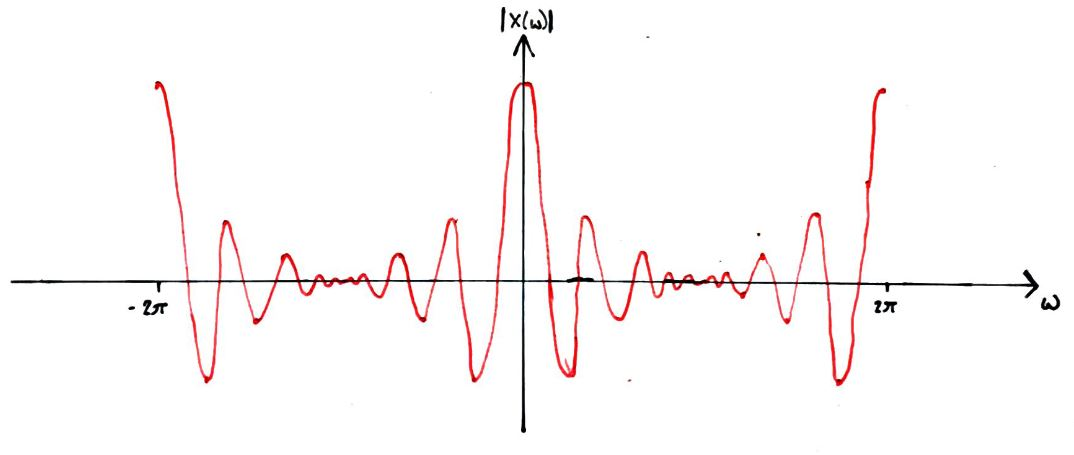
\includegraphics[width=\textwidth]{images/lecture_7_periodic_sinc.JPG}
  \caption{
  }
  \label{fig::lecture_7_periodic_sinc}
\end{figure}
%
We have seen for the continuous-time Fourier transform that
$x(t) * h(t) \Longleftrightarrow X(\omega)H(\omega)$. This still holds for the DTFT
as shown here:
%
\begin{align*}
  Y(\omega) &= \infsum{n}y[n]\ex{-\im\omega n} = \infsum{n}\infsum{k}x[k]h[n-k]\ex{-\im\omega n} \\
  &= \infsum{k}x[k]\infsum{n}h[n-k]\ex{-\im\omega n} = \infsum{k}x[k]\infsum{m}h[m]\ex{-\im\omega(m + k)} \\
  &= \infsum{k}x[k]\ex{-\im\omega k}\infsum{m}h[m]\ex{-\im\omega m} 
  = \infsum{k}x[k]\ex{-\im\omega k} H(\omega) \\
  &= X(\omega)H(\omega) \,.
\end{align*}

\subsection{Magnitude and Phase Responses}
%
\begin{exmp}
  Let $x[n] = a^n u[n]$ for $|a|>0$. Then,
  %
  \begin{displaymath}
    X(\omega) = \infsum{k}a^n u[n]\ex{-im\omega n} = \sum_{k=0}^\infty a^n\ex{-\im\omega n}
    = \sum_{n=0}^\infty\left(a\ex{-\im\omega}\right)^n \,.
  \end{displaymath}
  %
  This series is strictly decreasing, and so must be absolutely summable and
  hence can be represented by the DTFT. In this case, we have the geometric series
  %
  \begin{displaymath}
    X(\omega) = \sum_{n=0}^\infty\left(a\ex{-\im\omega}\right)^n = \frac{1}{1-a\ex{-\im\omega}} \,.
  \end{displaymath}
  %
  Note that this expression is complex-valued, and so we conclude as for the continuous
  time case that a real-valued signal yields a complex DTFT. It's convenient to be
  able to plot such complex-valued expressions, and so we plot the
  \textbf{magnitude response},
  %
  \begin{displaymath}
    |X(\omega)| = \left|\frac{1}{1-a\ex{-\im\omega}}\right|
    = \sqrt{\frac{1}{(1-a\ex{-\im\omega})(1-a\ex{\im\omega})}}
    = \frac{1}{\sqrt{1 + a^2 - 2a\cos(\omega)}} \,.
  \end{displaymath}
  %
  Some useful points on here include $|X(0)| = \frac{1}{1-a}$ and 
  $|X(\pm\pi)| = \frac{1}{1+a}$. The function resembles that of the frequency
  response of a decaying exponential as discussed in the previous lecture.
\end{exmp}
%
Typically, filters are named based on how their magnitude response looks. Some
``ideal filters'' are presented in Figure \ref{fig::lecture_7_ideal_filters}.
%
\begin{figure}[!htb]
  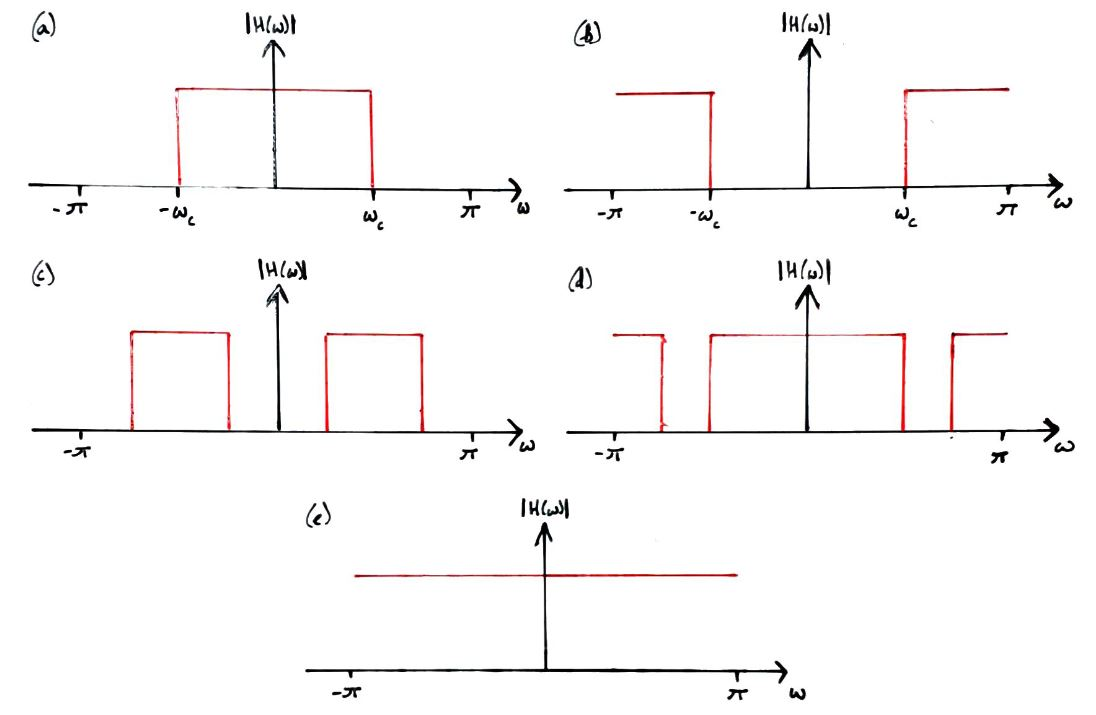
\includegraphics[width=\textwidth]{images/lecture_7_ideal_filters.JPG}
  \caption{
  }
  \label{fig::lecture_7_ideal_filters}
\end{figure}
%
The \textbf{phase response} is also an important quantity -- it transpires that
a desirable phase response is of the form $\theta = -c\omega$, where $c$ is some
constant. Consider a piecewise constant $\left|H(\omega)\right|$ as seen in
the ideal filters. In the pass region,
%
\begin{displaymath}
  Y(\omega) = H(\omega)X(\omega) = \left|H(\omega)\right|\ex{\im\theta}X(\omega) \,.
\end{displaymath}
%
Assuming that $|H(\omega)| = 1$,
%
\begin{displaymath}
  Y(\omega) = X(\omega)\ex{\im\theta} = X(\omega)\ex{-\im c\omega} \,,
\end{displaymath}
%
and transforming back to the time domain,
%
\begin{displaymath}
  y[n] = \frac{1}{2\pi}\int\dx{\omega}X(\omega)\ex{-\im c\omega}\ex{\im\omega n}
  = \frac{1}{2\pi}\int\dx{\omega}X(\omega)\ex{\im(n - c)\omega} = x[n-c] \,.
\end{displaymath}
%
In other words, this phase shift in the frequency domain becomes a delay in
the time domain. All frequencies are shifted by the same amount, and
so there's no distortion -- we have a pure delay of the input. But why can't we
have a zero delay? Recall that our ideal low pass filter in the time domain is
a $\sinc$, which is not causal, not absolutely summable (and consequently
not stable) and infinitely long. We'll find later that the introduction of a
delay (i.e. a non-zero phase) remedies these problems. For instance, we can
``kind of'' make the filter causal by shifting it in the time domain by some
constant $T$, such that the output at $t < 0$  is negligible. If we want to filter
a signal well, we have to tolerate some delay.
